%%% LaTeX Template: Article/Thesis/etc. with colored headings and special fonts
%%%
%%% Source: http://www.howtotex.com/
%%% Feel free to distribute this template, but please keep to referal to http://www.howtotex.com/ here.
%%% February 2011
%%%
%%% Last updated September 2018 by CDM

%%%  Preamble
\documentclass[11pt,letterpaper]{article}
\usepackage[margin=1.0in]{geometry}
\usepackage[T1]{fontenc}
\usepackage[bitstream-charter]{mathdesign}
\usepackage[latin1]{inputenc}					
\usepackage{amsmath}						
\usepackage{xcolor}
\usepackage{cite}
\usepackage{hyphenat}
\usepackage{graphicx}
\usepackage{float}
\usepackage{subfigure}
\usepackage{sectsty}
\usepackage[compact]{titlesec} 
\usepackage[tablegrid]{vhistory}
\allsectionsfont{\color{accentcolor}\scshape\selectfont}

%%% Definitions
\definecolor{accentcolor}{rgb}{0.0,0.0,0.5} 
\newcommand{\teamname}{Team Name}
\newcommand{\productname}{Product Name}
\newcommand{\coursename}{CSE 4316: Senior Design I}
\newcommand{\semester}{Spring 2019}
\newcommand{\docname}{Project Charter}
\newcommand{\department}{Department of Computer Science \& Engineering}
\newcommand{\university}{The University of Texas at Arlington}
\newcommand{\authors}{Utsab Acharya \\ Sudip Kandel \\ Sandesh Naga \\ Bhaskar Acharya \\ Tara Gurung}

%%% Headers and footers
\usepackage{fancyhdr}
	\pagestyle{fancy}						% Enabling the custom headers/footers
\usepackage{lastpage}	
	% Header (empty)
	\lhead{}
	\chead{}
	\rhead{}
	% Footer
	\lfoot{\footnotesize \teamname \ - \semester}
	\cfoot{}
	\rfoot{\footnotesize page \thepage\ of \pageref{LastPage}}	% "Page 1 of 2"
	\renewcommand{\headrulewidth}{0.0pt}
	\renewcommand{\footrulewidth}{0.4pt}

%%% Change the abstract environment
\usepackage[runin]{abstract}			% runin option for a run-in title
%\setlength\absleftindent{30pt}			% left margin
%\setlength\absrightindent{30pt}		% right margin
\abslabeldelim{\quad}	
\setlength{\abstitleskip}{-10pt}
\renewcommand{\abstractname}{}
\renewcommand{\abstracttextfont}{\color{accentcolor} \small \slshape}	% slanted text

%%% Start of the document
\begin{document}

%%% Cover sheet
{\centering \huge \color{accentcolor} \sc \textbf{\department \\ \university} \par}
\vspace{1 in}
{\centering \huge \color{accentcolor} \sc \textbf{\docname \\ \coursename \\ \semester} \par}
\vspace{0.5 in}
\begin{figure}[h!]
	\centering
   	
\includegraphics[width=0.60\textwidth]{images/test_image}
\end{figure}
\vspace{0.5 in}
{\centering \huge \color{accentcolor} \sc \textbf{\teamname \\ \productname} \par}
\vspace{0.5 in}
{\centering \large \sc \textbf{\authors} \par}
\newpage


%\vspace{1 in}
%\centerline{January 13th, 2012}
%\newpage

%%% Revision History
\begin{versionhistory}
  	\vhEntry{0.1}{10.01.2018}{GH}{document creation}
  	\vhEntry{0.2}{10.05.2018}{AT|GH}{complete draft}
  	\vhEntry{0.3}{10.12.2018}{AT|GH}{release candidate 1}
  	\vhEntry{1.0}{10.20.2018}{AT|GH|CB}{official release}
  	\vhEntry{1.1}{10.31.2018}{AL}{added customer change requests}
\end{versionhistory}
\newpage

%%% Table of contents
\tableofcontents
\newpage

%%% List of figures and tables (optional)
\listoffigures
%\listoftables
\newpage
\setcounter{table}{0}

%%% Agile project charter sections
\section{Vision}
The vision defines the "Why" of the project. This is the higher purpose, or the reason for the project’s existence. This section should avoid mentioning implementation details, and focus more on what the current problem is and what would be gained if the problem were to be solved. 

\section{Mission}
fgfgf This is the "What" of the project and it states what will be done in the project to achieve its higher purpose (the higher purpose being the vision” discussed above). This section should focus mostly on what your solution is going to be and what it is going to do.
\section{Success Criteria}
The success criteria are enumerated effects outside of the development of the solution (i.e., NOT specific project requirements) that can be observed and measured to quantify "what success looks like". The key is to focus on specific expected benefits beginning immediately after the project is delivered and projecting forward into the future. Bullet lists should be used to itemize each success criterion, and each item should have a time frame and some sort of quantifiable measurement.

One way to list the success criteria is to use lists for different time frames. Here is a short example:
\\
\\
Upon completion of the prototype system, we expect the following success indicators to be observed on kiosk stations implementing the new GUI software:
\begin{itemize}
  \item A 10\% reduction in operating costs
  \item 30\% reduction in average transaction time
  \item 20\% increase in mean time to failure (MTTF)
\end{itemize}

Within 6 months after the prototype delivery date, we expect the following success indicators to be observed:
\begin{itemize}
  \item An additional 10\% reduction in operating costs
  \item An additional 10\% reduction in average transaction time
  \item An additional 5\% increase in mean time to failure (MTTF)
\end{itemize}

Within 12 months after the prototype delivery date, we expect the following success indicators to be observed:
\begin{itemize}
  \item Expansion of the system to 3 additional deployment sites
  \item Porting of the system to additional hardware platforms, such as Super Kiosk and Alpha Pay
  \item An additional 15\% reduction in operating costs
\end{itemize}
\\
\\
NOTE: The vision, mission, and success criteria, when combined, should occupy \underline{EXACTLY ONE FULL PAGE}. This can be individually distributed as an agile project charter or executive summary when necessary. 
\\
NOTE: Throughout the document, remove and replace all instruction text with your own material. 

\newpage

%%% Remaining project charter sections
\section{Background}
The main objective of this application is to help people record what they own in the organized fashion. We people are surrounded by lots of items like food, drinks, collectibles and much more. The main problem is not finding what is needed at the specific time. Our app will help people store the information about the location and specific attributes about the items or products that they have and retrieve it when needed without having the hassle to remember where you left it last. Similarly, when you own a lot of stuffs you don't remember if the things that you own is going to go bad within a week or couple of months. Our app will notify users about the goods that are going to go bad in near future. Similarly, we are creating the app for free. Lots of app that are available in the market right now are the paid apps. Our app will be like a personal assistant who knows where items are stored and is also smart when it comes to the expiry of items and more.
\section{Related Work}
There are several numbers of inventory apps commercially available for use. Different people have built the apps in different ways. Some apps perform really well whereas some other apps are not as promising as it looks.There are several apps that I looked at. one of the very first app that I looked at was \textbf{Inventory+ from Mostafa Ashour, Tryvin}. This app was priced at 4.99 dollars but it failed to implement even very basic features like bar code scan support, easy removal and addition of the item. Similarly another app that I looked on was \textbf{Inventory Control with Scanner by Starkode Limited Company}. As I researched I found the app to be slow and very buggy. Looking at the reviews lots of users were complaining about the app often crashing.\textbf{ Cashier by cashier live} was another app that i researched about. It is an inventory app integrated with the POS system. The app cost was $75$ per month. I tried out one of my friends copy but the app was very laggy. It was slow and creating a user feature was not working at that particular time. \textbf{myStock Inventory Manager by Trace Width Technology Solutions LLC.} is another app that I tried. This time the app was not reliable. It had trouble loading the items. Sync between two device is really poor. Similarly another app I used was \textbf{Inventory app - Zoho by zoho corporation}. The app was completely functional and it the one app that i like the most. \\
All these apps provide the basic functionality of storing and retriving information. Most of the apps are paid applications. These type of app does not work for our client because non of these apps store the location of the item. Upon entry non of the apps will ask for the preferred location for storage nor it provides the items location on retrieval. Also most of the apps are slow and unreliable. We want to provide something robust and easy to use to our customer.
\section{System Overview}
Our app will be mobile based app that can run both on android as well as ios operating system. We are going to implement a simple user interface where a user can interact and perform all necessary tasks within the app with ease. Basically, at high level our user wants to store something safely where he won't forget. We help user do just that with the help of our app. First, We let the user to define the area where he would like to store his item. Then we let him store the item in the storage and then we will record the information about the item in the database, and retrieve it when it is needed. User will be able to use his camera for scanning the item, he does not have to manually enter every detail about the item that he wants to store. Similarly, once the user scans the picture of the item we will store items information in the database with its specific information. When he wants to retrieve the item he can simply search for the item in the app and the app will tell him where he stored the item, when and what are the important information about the item that he needs to know. for example the item is something that expires, the app will tell the user that it is going to expire on this date once searched. Also, if something is not searched and its expiry date is near then also the app will automatically notify the user about its expiry date. 
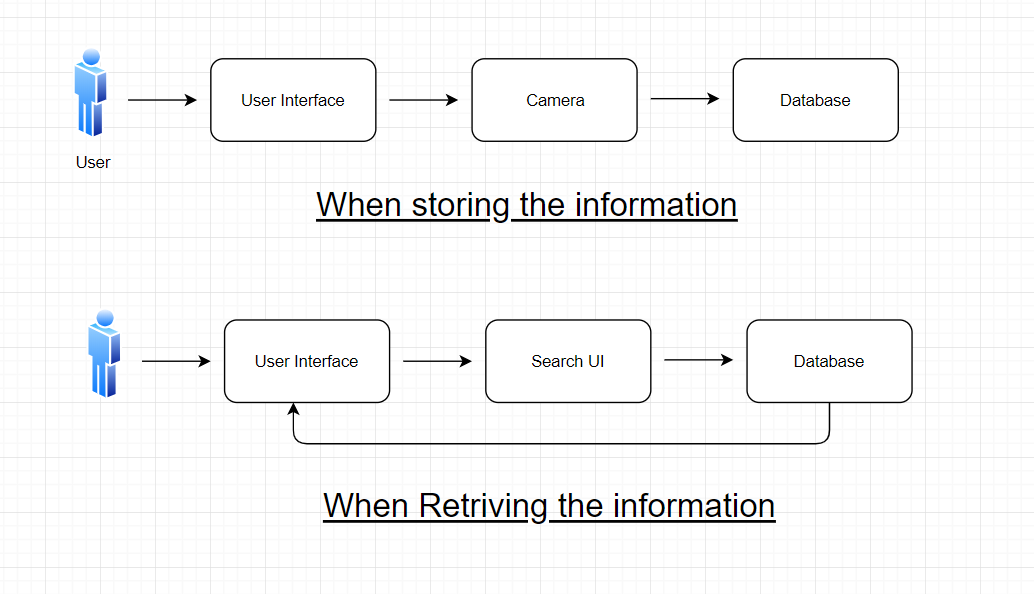
\includegraphics{project charter latex/images/component.PNG}
\section{Roles \& Responsibilities}
Who are the stakeholders of the project? Who will be the point of contact from the sponsor or customer side? Who are the team members, and what will be their areas of responsibility? Will your team maintain the product owner and scrum master for the whole project, or will that role change periodically? This section should occupy 1/2 - 1 full page.
\section{Cost Proposal}
This section contains the approximate budget for the project, where that money will come from, and any other support. This text should be replaced with a discussion and justification of major expenses, but not the actual monetary amounts (that will go in the preliminary budget section below). 

\subsection{Preliminary Budget}
Include a high level budget table for components, fabrication, software licensees, development hardware, etc. 

\subsection{Current \& Pending Support}
What are all of the funding sources for the project, and are there any potential funding sources that haven't been secured yet? List all funding sources (including the default funding amount provided by the CSE department) and their dollar amounts.
\section{Facilities \& Equipment}
What lab space, testing grounds, makerspaces, etc. will you need to complete the project? Will you require any specific equipment, and if so, where will you get it (borrow, lease, purchase, outsource, already present in the lab, etc.). This section should occupy 1/2 page.
\section{Assumptions}
An assumption is a belief of what you assume to be true in the future. You make assumptions based on your knowledge, experience or the information available on hand. These are anticipated events or circumstances that are expected to occur during your project's life cycle.

Assumptions are supposed to be true but do not necessarily end up being true. Sometimes they may turn out to be false, which can affect your project significantly. They add risks to the project because they may or may not be true. For example, if you are working on an outdoor unmanned vehicle, are you assuming that testing space will be available when needed? Are you relying on an external team or contractor to provide a certain subsystem on time? If you are working at a customer facility or deploying on their computing infrastructure, are you assuming you will be granted physical access or network credentials?

This section should contain a list of at least 5 of the most critical assumptions related to your project. For example:

The following list contains critical assumptions related to the implementation and testing of the project.

\begin{itemize}
  \item A suitable outdoor testing location will be available by the 3rd sprint cycle
  \item The X sensing system developed by Sensor Consulting Company will be delivered according to specifications by the 4th sprint cycle
  \item Access to the customer installation site will be provided by the 5th sprint cycle
  \item The customer will provide ample power and network connectivity at the installation site
  \item The installation site network infrastructure will allow TCP network traffic on port 8080
\end{itemize}
\section{Constraints}
Constraints are limitations imposed on the project, such as the limitation of cost, schedule, or resources, and you have to work within the boundaries restricted by these constraints. All projects have constraints, which are defined and identified at the beginning of the project.

Constraints are outside of your control. They are imposed upon you by your client, organization, government regulations, availability of resources, etc. Occasionally, identified constraints turn out to be false. This is often beneficial to the development team, since it removes items that could potentially affect progress.

This section should contain a list of at least 5 of the most critical constraints related to your project. For example:

The following list contains key constraints related to the implementation and testing of the project.

\begin{itemize}
  \item Final prototype demonstration must be completed by May 1st, 20XX
  \item The customer will provide no more than two maintenance personnel to assist in on-site installation
  \item Customer installation site will only be accessible by development team during normal business hours
  \item Total development costs must not exceed \$800
  \item All data obtained from customer site must be reviewed and approved for release by the Information Security Office prior to being copied to any internet connected storage medium
\end{itemize}

\section{Risks}
This section should contain a list of at least 5 of the most critical risks related to your project. Additionally, the probability of occurrence, size of loss, and risk exposure should be listed. For size of loss, express units as the number of days by which the project schedule would be delayed. For risk exposure, multiply the size of loss by the probability of occurrence to obtain the exposure in days. For example:

The following high-level risk census contains identified project risks with the highest exposure. Mitigation strategies will be discussed in future planning sessions.

\begin{table}[h]
\resizebox{\textwidth}{!}{
\begin{tabular}{|l|l|l|l|}
\hline
 \textbf{Risk description} & \textbf{Probability} & \textbf{Loss (days)} & \textbf{Exposure (days)} \\ \hline
 Availability of X sensor module due to contractor delay  & 0.50 & 20 & 10 \\ \hline
 Outdoor testing grounds are not available  & 0.20 & 14 & 2.8 \\ \hline
 Internet access not available at installation site  & 0.30 & 9 & 2.7 \\ \hline
 Delays in shipping from overseas vendors  & 0.10 & 20 & 2.0 \\ \hline
 Certification delays at compliance testing facility & 0.15 & 10 & 1.5 \\ \hline
\end{tabular}}
\caption{Overview of highest exposure project risks} 
\end{table}
\section{Documentation \& Reporting}
%%% In this section, you will describe all of the various artifacts that you will generate and maintain during the project life cycle. Describe the purpose of each item below, how the content will be generated, where it will be stored, how often it will be updated, etc. Replace the default text for each section with your own description. Reword this paragraph as appropriate.

\subsection{Major Documentation Deliverables}

\subsubsection{Project Charter}
A project charter is the statement of scope, objectives and people who are participating in a project. It begins the process of defining the roles and responsibilities of those participants and outlines the objectives and goals of the project. The charter also identifies the main stakeholders and defines the authority of the project manager.
Project Charter for this project is uploaded in overleaf, and it is made available to all the group member and all of them will have access to modify or update any required content with all group approval.  

\subsubsection{System Requirements Specification}
System Requirement Specifications are kept as a doc file and is made available in google doc. All requirements are collected in that doc file and each addition of the requirements is made with group discussions and are prioritized on the basis of functionalities they required and the usefulness of that requirement to make our application more applicable and worthy.

\subsubsection{Architectural Design Specification}
The system is designed using the Object Oriented architectural style. As it provide a high-level overview of how the functionality and responsibilities of the system were partitioned and then assigned to subsystems or components. This document is also  The overall architecture is a Event driven using the React Native framework. The system consists of the Client component, Database component and all set of rules to be executed base of the events created by user and notify the user. 


\subsubsection{Detailed Design Specification}
    Core feature of our application will work as shown below
    \begin{figure}[h!]
        \centering
        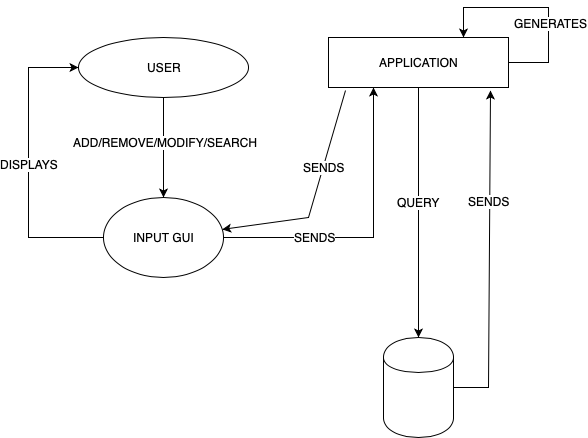
\includegraphics[width=.5\textwidth]{images/core}
        \caption{Informal-Data Flow}
    \end{figure}


\subsection{Recurring Sprint Items}
\subsubsection{Product Backlog}
The product backlog is a kind of living document, as it keeps changing on the basis of the feature being added and the requirement of the system. Each entry on the product backlog as so designed that it will add value for the customer. Product backlog main consist of the  list of all things that needs to be done within the project. It replaces the traditional requirements specification artifacts. Scrum master is responsible for keeping the product backlog up to date with the discussion to the group mate as we are the product owners. We will be using spreed-sheet to maintain the product back log and will be using google doc to share it with all team members. 

\subsubsection{Sprint Planning}
As we have our own system, all the team members will be discussing about the features of the application and all the requirements, and all the sprint goals will be updated in the spreed sheet. A scrum master or coach typically facilitates sprint planning in order to ensure that the discussion is effective and that there is agreement to the sprint goal and that the appropriate product backlog items are included in the sprint backlog. Generally to complete our project our team will required no more that 10-11 sprints.

\subsubsection{Sprint Goal}
Each of the team member is responsible achieve the spring goal. As the scrum master the assigned the task to the individual, its their duty to complete that task in given time frame so that it won't affect other team, who are depend upon the completion of the given task for next phase of sprint cycle. As it is our own product no customer involvement is necessary but as a consumer we will be consulting couple of our friends for feedback on our features implemented in each sprint cycle.  

\subsubsection{Sprint Backlog}
Each meeting will cover the task that are do and the remaining task. All the task are kept in the form of spreadsheet, so its easier for everybody to keep track of the system progress. once all the remaining task is decided, scrum master will be assigning the task to each of the team member including him/her. 

\subsubsection{Task Breakdown}
As we are building our own product, the scrum master will be responsible to divide the task to be completed in that sprint cycle and based on the field of as individual, scrum master will assign the work and s/he will keep the record of assigned task and individual are obliged to give the progress report on the daily basic to the scrum master.


\subsubsection{Sprint Burn Down Charts}
On each sprint cycle one of the group member is assigned as a team leader(scrum master) who will note down every progress report of all team members and s/he will be responsible to make the sprint burn down chart based on the assigned work to the team members and due dates. As each task will assigned certain points,i.e harder the task more points it carries and individual will report his/her daily progress to the team leader and based on that team leader will generate the excel chart to generate the burn down chart for each sprint. As all the materials is made available in google doc, if some mistakes are done by anybody, other group member can correct it.  

                   \begin{figure}[!h]
                        \centering
                        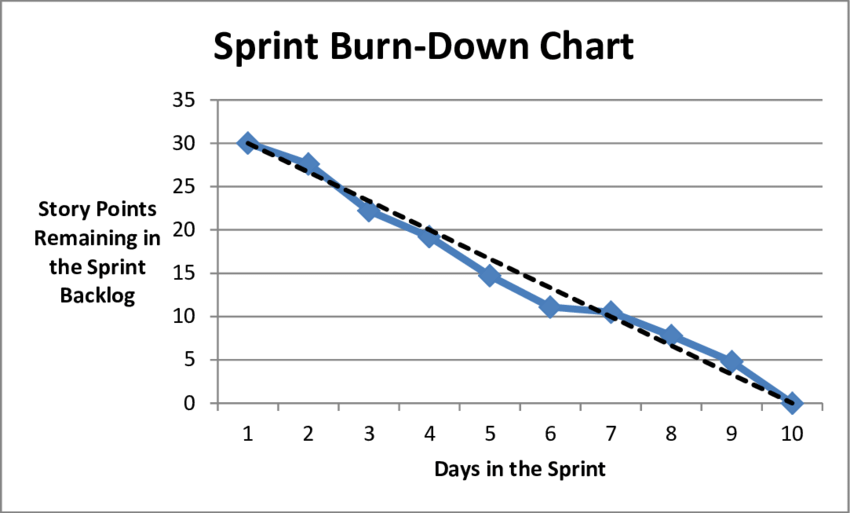
\includegraphics[width=0.5\textwidth]{images/burn}
                        \caption{Example sprint burn down chart \cite{Anon2019}}
                    \end{figure}
                   

\subsubsection{Sprint Retrospective}
Our every team discussion are written in our ENB with exact time and date, title of discussions, ideas created, decisions taken and reasons of selection of that specific decision. So if any of us wants to look back about why we took that decision can refer to ENB. Even though our ENB will be individual, almost all the content inside will be similar because every suggestions and things will be noted there, regardless whose opinion is that. This note taking process continues as our meeting starts and will end after couple aof minutes after meeting ends in order to give individual to note down the missing part from the peers. 


\subsubsection{Individual Status Reports}
On each sprint meeting each member will be assigned task to do with the due dates, and our team leader at that specific time will responsible to keep track of everyone in the team and keep record of quality of result produced by the team member in that given specific time. At the end of each sprint cycle team leader is responsible to submit the individual status report to the professor in-order to give the picture about how team is doing.


\subsubsection{Engineering Notebooks}
Engineering Notebooks is one of the efficient, easy way of keeping track of progress and counted as the legal form, if any legal issue occurs. So we will be updating our notebook on every meeting, and truly the number of pages will depend upon the ideas, each of the team member comes up with. Our ENB will be signed as a "witness" by our professor.   


\subsection{Closeout Materials}


\subsubsection{System Prototype}
Basically our final project is the full functioning mobile application. So we will allow any user to do testing on their phone and more than happy to get feedback for the improvement. We will be demonstrating our final project early fall 2019. 


\subsubsection{Web Page}
Out project web page will include the introduction to our application, its all of the features. Our targeted consumer, all the developers name with their linked profile. And we will keep updating our application as the requirements increases and will announce all the releases in the web page.


\subsubsection{Demo Video}
In our demo we will be using a well functioning application from our phone to do various task which include its core features. Our demo might takes about 8-10 minutes.


\subsubsection{Source Code}
All of our team members are familiar with GitHub and had done several project using it as a version control system, we had decided to use it as our version control tool. All the repository created will be private and no source code will be provide to the customer. As we planed to deploy out final application to the apple store, its free to use for public. All out license term and condition will be listed in a single readme file.


\subsubsection{Source Code Documentation}
Almost all  of the documentation are generated using latex and we will be using overleaf as a leTex editor, our final documentation will be provided in PDF format



\subsubsection{Installation Scripts}
Once our application is deployed in the app store, user will be able to search the app from their play store on their and can install it for free of cost.

\subsubsection{User Manual}
User will be have access to click the help option from the menu bar in the application itself, which will teach the steps to be able to use the various feature of the application.

\newpage

%%% References
\bibliographystyle{plain}
\bibliographystyle{reference/IEEEtran_custom}
\bibliography{reference/refs}{}

\end{document}